% Prof. Dr. Ausberto S. Castro Vera
% UENF - CCT - LCMAT - Curso de Ci\^{e}ncia da Computa\c{c}\~{a}o
% Campos, RJ,  2023
% Disciplina: Paradigmas de Linguagens de Programa\c{c}\~{a}o
% Aluno: Gabriel Costa Fassarella


\chapterimage{ScalaH} % Chapter heading image
	
	%%%---------------------------------------------
	\chapter{Scala: A Programação Em Alta Performance }
	
	%%%---------------------------------------------
	\section{Introdução}
	Neste capítulo, trataremos sobre os principais aspectos da linguagem de programação Scala segundo os conceitos propostos pelos autores \cite{Odersky}, \cite{Sfregola2021} e \cite{Wampler2021}. De acordo com \cite{Sfregola2021} Scala é uma linguagem de programação funcional e orientada a objetos que durante os últimos anos vem crescendo em popularidade entre inúmeros desenvolvedores. O fato da Scala usar  multiparadigmas faz com que sua eficiência, capacidade de lidar com projetos de grande porte e legibilidade sejam algumas de suas principais características. A linguagem usa dois tipos de paradigmas de programação: a programação orientada a objetos e ainda utiliza programação funcional. 
	
	Segundo \cite{Sfregola2021}: "a abordagem orientada a objetos pode
	ser mais eficiente, mas propenso a erros. Ao usar o estado mutável, seu programa realocará sua memória: toda vez que ocorrer uma alteração, ele alterará o
	dados no lugar. No entanto, o estado de compartilhamento pode fazer com que seu aplicativo sofra problemas de inconsistência de dados devido a vários processos acessando e modificando a mesma porção de dados", ou seja, o uso da linguagem orientada a objetos pode apresentar uma boa performance, porém pode gerar uma boa quantidade de erros, já que é comum que nesse paradigma o programa receba diversas realocações de memória, mudando assim a localização dos dados, fazendo com que possam surgir problemas na data utilizada. Já a programação funcional pode garantir uma melhor legibilidade, já que por apresentar dados imutáveis o compartilhamento é mais seguro. Porém, esse paradigma apresenta uma menor performance, uma vez que o seu uso de memória costuma ser alto, já que a atualização de variáveis não é recorrente na programação funcional.
	
	%%%---------------------------------------------
	\section{História}
	
	Scala foi fundada em 2002 pelo professor Martin Odersky (imagem abaixo) e sua equipe em uma escola politécnica da Suíça, a École Polytechnique Fédérale de Lausanne (EPFL). Ainda em 1995, Odersky decidiu estudar o Java, e passou a se interessar em criar uma linguagem que usasse o paradigma de programação funcional. Isso fez com que ele se juntasse com Philip Wadler em uma equipe para criar uma linguagem funcional que fosse compilada para o Java Bytecode. Esse trabalho em conjunto, pouco tempo depois deu origem ao compilador Pizza.
	
	\begin{figure}[H]
		\centering
		
\includegraphics[width=8cm]{Pictures/Odersky}
		\caption{}
		\label{fig:odersky}
		Fonte: \href{https://twitter.com/odersky?s=20}{Twitter de Odersky}
	\end{figure} 
	
	O seu trabalho com o Pizza fez com que em 1997 ele entrasse em contato com a equipe de desenvolvedores da Sun Microsystems. O que permitiu a sua participação no desenvolvimento do Generic Java (GJ), um novo compilador javac. Segundo \cite{Venners} em uma entrevista com o próprio Martin Odersky \href{https://www.artima.com/articles/the-origins-of-scala}{disponível aqui}: "Foi emocionante trabalhar em Java por causa de seu enorme impacto, mas também foi muito difícil porque Java é uma linguagem rica com muitos recursos que muitas vezes entram em conflito com extensões de maneiras imprevistas."
	
	Em 1999, Odersky passou a lecionar na EPEL, e assim se sentiu livre para começar a criar o projeto de uma linguagem que unisse a programação orientada a objetos e programação funcional sem as limitações impostas pelo Java. Com essa ideia em mente, ele criou o Funnel, uma linguagem descrita por ele em \cite{Venners} como: "lindamente simples, com muito poucos recursos de linguagem primitiva" criada para a utilização em redes funcionais. Porém, o uso da linguagem não se mostrou tão eficaz, já que o minimalismo apresentado pela linguagem trazia dificuldades para novos usuários, e para os mais experientes se tornava uma tarefa entediante ter que executar as mesmas linhas de código diversas vezes.
	
	Tal cenário fez com que fosse necessária a criação de uma linguagem que apresentasse uma grande quantia de bibliotecas padrões. Isso fez com que Odersky começasse a trabalhar na linguagem Scala em 2001, até o seu primeiro lançamento em 2003. Segundo Martin Odersky, Scala foi criado não com o intuito de ser uma extensão do Java, mas sim uma linguagem totalmente integrada com ele, já que Scala é traduzido para um Bytecode de java. Segundo Odersky em \cite{Venners}: "Scala foi projetado para ser orientado a objetos e funcional. É uma linguagem puramente orientada a objetos no sentido de que todo valor é um objeto. Objetos são definidos por classes, que podem ser compostas usando composição mixin. Scala também é uma linguagem funcional no sentido de que toda função é um valor. As funções podem ser aninhadas e podem operar em dados usando correspondência de padrões."
	
	
	
	
	%%%---------------------------------------------
	\section{JVM e SBT}
	Uma linguagem orientada a objetos com tipagem estática, como o Scala, tem como característica a verificação dos tipos de dados durante a compilação. Ou seja, se existe um dado do tipo float, apenas operações do tipo float serão permitidas com esse dado, evitando uma série de erros, uma vez que esses bugs podem ser contidos durante o processo de compilação. Porém para isso, é necessário utilizar a JVM (Java Virtual Machine), uma máquina virtual usada para executar uma sequência de instruções denominadas Bytecode.
	
	\begin{figure}[H]
		\centering
		\caption{Funcionamento JVM}
		\label{Byte Code}
		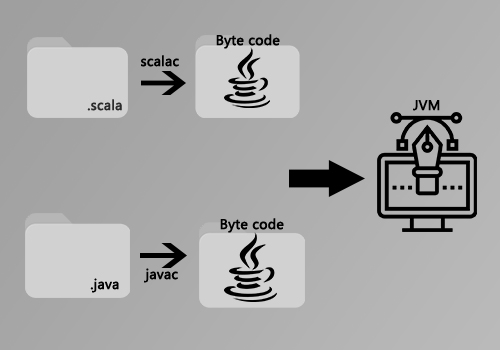
\includegraphics[width=10cm]{JVM.jpg} \\
		Fonte: Autor
	\end{figure}
	
	De acordo com \cite{Sfregola2021}: "A JVM é uma máquina para realizar tarefas executando um conjunto bem definido de operações, chamadas de bytecode. Uma linguagem JVM visa traduzir seu código em executável Bytecode JVM, geralmente formado por vários arquivos com extensão *.class. Ao codificar em Java, você salva seus arquivos fonte com extensão *.java e usa o compilador javac para produzir um arquivo jar contendo o bytecode gerado", ou seja, quando um usuário está programando em Java, e deseja executar um arquivo, é necessário que o mesmo seja salvo utilizando a extensão .java, para que assim o compilador  javac possa ser usado para criar um arquivo java que possua o bytecode que deverá ser traduzido para código de máquina nativo pela JVM, dessa forma executando as instruções desejadas. Algo semelhante ocorre com Scala, o usuário deve salvar o arquivo usando a extensão .scala, isso faz com que o compilador scalac crie um arquivo scala que possua o bytecode, e por sua vez seja utilizado pela JVM para executar as instruções. Além desse processo, a JVM é responsável por outras funções, como verificar a integridade de um arquivo bytecode, organizar e a memória do código e gerenciar os processos.
	
	A JVM foi criada com o intuito de ofertar ao usuário uma plataforma independente para a execução de seus programas, isso faz com que esses códigos possam ser executados em qualquer sistema operacional, desde que ele tenha suporte para a JVM. Esse cenário faz com que linguagens que utilizem a JVM, sejam extremamente populares na programação de multiplataformas.
	
	Com isso, tornou-se necessária a criação de uma ferramenta que facilitasse a construção, empacotamento e compilação de códigos em Scala. Para isso foi criado o SBT (Simple Build Tool), de acordo com \cite{Sfregola2021}: "sbt é a ferramenta de construção mais comum na comunidade. É um complexo, mas poderoso ferramenta que gerencia suas dependências e define o ciclo de construção do seu código", ou seja, ela é uma ferramenta associada a linguagem, responsável por gerenciar os projetos em Scala, podendo gerar desde documentações até executar alguns testes automatizados, além de outras operações necessárias para a construção de um código.
	
	Utilizando o SBT é possível que o usuário possa automatizar tarefas mais comuns do Scala, fazendo com que o processo de desenvolvimento do código seja mais fácil e eficiente. Isso faz com que essa ferramenta seja extremamente utilizada pela comunidade Scala, e é considerada como uma ferramenta indispensável para os desenvolvedores que usam a linguagem.
	
	%%%---------------------------------------------
	\section{Aplicações}
	Scala é uma línguagem extremamente moderna e versátil, que pode ser usada para inúmeras aplicações diferentes, seja pela sua segurança, performance, ampla variedade de bibliotecas ou compatibilidade com outras linguagens, fazendo com que diversas áreas diferentes possam optar pela utilização da Scala em seus códigos. Alguns exemplos de aplicações da linguagem são:
	
		%%%---------------------------------------------
		\subsection{Desenvolvimento Web}
		Como demonstrado na figura abaixo, a área do desenvolvimento Web pode abranger uma vasta rede de categorias diferentes. Por esse motivo Scala costuma ser amplamente utilizada na produção de web aplicativos de alta performance. Isso ocorre pois Scala é uma linguagem de alto nível orientada a objetos, e seus projetos apresentam uma uma grande efetividade, uma vez que ela foi feita para ser executada em tempo real pelo compilador, acelerando assim o tempo de processamento do código. 
		
		\begin{figure}[H]
			\centering
			
\includegraphics[width=0.7\linewidth]{Pictures/DesenWeb}
			\caption{}
			\label{fig:desenweb}
			Fonte: \href{https://www.pngwing.com/pt}{PNG Wing}
		\end{figure}
		
		A compatibilidade do Scala com Java e outras linguagens de programação é um importante fator no uso da linguagem nessa área, uma vez que essa característica permite o uso de bibliotecas e frameworks java, podendo ainda aproveitar o uso da sintaxe breve apresentada pela linguagem. Tal situação possibilita uma maior liberdade e facilidade ao desenvolvedor na utilização do Scala em seus projetos.
		
		Outro fator fundamental para a utilização do Scala em desenvolvimento web é a presença da modularidade e escalabilidade, que permitem a criação de projetos complexos. A programação assíncrona é extremamente importante para isso, uma vez que ela permite que os programadores criem códigos assíncronos de maneira segura.
		
		%%%---------------------------------------------
		 \subsection{Big Data}
		 Como ilustrado na imagem abaixo, Big Data é uma área que envolve um imenso fluxo de dados diferentes. Por isso Scala é uma linguagem muito utilizada na manipulação de big data, podendo processar uma grande quantia de dados em tempo real. Isso ocorre porque a linguagem foi adaptada para lidar com um enorme volume de informações, por meio da programação funcional, modularidade e escalabilidade apresentada pela Scala. Isso ainda permite ao programador uma maior flexibilidade e uma programação mais abrangente, já que a Scala é uma linguagem de multiparadigmas. 
		 
		\begin{figure}[H]
			\centering
			
\includegraphics[width=0.7\linewidth]{Pictures/BigData}
			\caption{}
			\label{fig:bigdata}
			Fonte: \href{https://www.pngwing.com/pt}{PNG Wing}
		\end{figure}
		
		Além disso, a linguagem foi feita para ter um suporte de programação assíncrona e paralela, ou seja, o programa executa múltiplas tarefas de uma só vez, mas de maneiras diferentes. Isso permite que tarefas possam ser executadas em paralelo, permitindo o aumento da velocidade de processamento dos dados apresentados. 
		
		Scala ainda é uma linguagem de programação que apresenta uma sintaxe sólida e breve, isso permite que a aplicação de projetos para big data sejam extremamente simplificados, já que os programadores podem escrever menos código e realizar mais funções, acelerando o processo e custo de desenvolvimento, podendo ainda escrever códigos eficientes e de alto desempenho. 
		
		 %%%---------------------------------------------
		 \subsection{Softwares Empresariais}
		 Como ilustrado na imagem abaixo, empresas costumam lidar com uma grande quantia de usuários gerenciando os seus sistemas de inúmeras maneiras. Por esse motivo o Scala pode ser usado para o desenvolvimento de softwares empresariais que exigem aplicativos escaláveis, uma vez que, em alguns casos, essas empresas necessitam de softwares que tratem com uma enorme quantia de dados e/ou trafego de usuários, e isso permite que a linguagem acompanhe o crescimento da empresa, e como já dito antes, a imutabilidade garante a segurança dessa data.
		 
		\begin{figure}[H]
			\centering
			
\includegraphics[width=0.7\linewidth]{Pictures/Empresario}
			\caption{}
			\label{fig:empresario}
			Fonte: \href{https://www.pngwing.com/pt}{PNG Wing}
		\end{figure}
		
		Como já citado anteriormente, a possibilidade da programação assíncrona e em paralelo permite que os dados sejam processados mais rapidamente. Tal cenário junto com a utilização da JVM (que permite uma otimização de desempenho) faz com que a linguagem tenha uma grande vantagem para o mercado, já que o fluxo de dados em empresas (especialmente nas de grande porte) é extremamente alto.
		
		Além disso, o fato de que Scala é uma linguagem com multiparadigmas faz que ela seja uma extremamente versátil e adaptável, podendo ser usada para inúmeras necessidades que uma empresa exige diariamente, permitindo ainda a construção de códigos eficientes e alto desempenho. 
		
	%%%---------------------------------------------